% Adapted from [MaYo26].  Regenerate: see README.md in this directory.
\documentclass[border=6pt,varwidth=17cm]{standalone}
%% Shared preamble for the figures adapted from [MaYo26]
%% (T. Makino and T. Yokoyama, RC 2026, LNCS 16626).  Copied from the
%% authors' own LaTeX source of that paper.
\usepackage[T1]{fontenc}
\usepackage{stmaryrd}
\newcommand{\sem}[1]{\llbracket #1 \rrbracket}
\usepackage{amsmath}
\usepackage{amssymb}
\usepackage{xcolor}
\pagecolor{white}
\def\pgfsysdriver{pgfsys-dvisvgm.def}
\usepackage{tikz}
\usetikzlibrary{shapes.geometric, positioning,calc}
\tikzset{
  label/.style={font=\footnotesize, font=\ttfamily},
  labelA/.style={font=\footnotesize},
  code/.style={font=\footnotesize, font=\ttfamily, text=gray},
  proc/.style={rectangle, draw, minimum size=1cm, text centered, dashed, font=\ttfamily},
  test/.style={diamond, draw, minimum size=1cm, aspect=1, text centered, font=\ttfamily},
  assert/.style={diamond, draw, minimum size=1cm, text centered, font=\ttfamily},
  asn/.style={rectangle, draw, minimum size=.5cm, text centered, font=\ttfamily},
  >=latex,
  terminal/.style={rectangle, rounded corners, draw, minimum height=6mm, text centered},
}
\renewcommand{\t}[1]{\texttt{#1}}
\newcommand{\tm}[1]{\mathtt{#1}}

\begin{document}
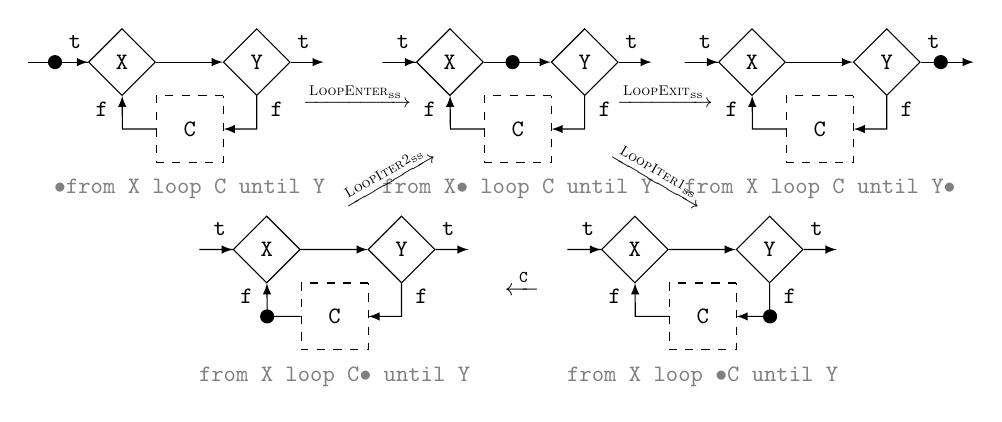
\begin{tikzpicture}[scale=.85, transform shape]
  \fill (-1, 0) circle (3pt);
  \node[assert] (X) at (0, 0) {X}; %
  \node[test, right=of X] (Y) {Y};
  \node[proc] (C) at ($(Y)+(-1, -1)$) {C};
  \draw[->] (X) -- ++(-1.4, 0) -- (X);
  \node[label] at ($(X)+(-.7, .3)$) {t}; %
  \draw[->] (X) -- (Y);
  \draw[->] (Y) -- ++(1, 0);
  \node[label] at ($(Y)+(.7, .3)$) {t}; %
  \draw[->] (Y) -- ++(0,-1) -- ++(-0.4,0) -- (C);
  \node[label] at ($(Y)+(.3, -.7)$) {f}; %
  \draw[->] (C.west) -- ++(-.5, 0) coordinate (temp) -- (X);
  \node[label] at ($(X)+(-.3, -.7)$) {f};
  \node[code] at ($(C)+(0, -.9)$) {$\bullet$from X loop C until Y};

  \node[labelA] at ($(Y)+(1.5, -.5)$) {$\xrightarrow{\textsc{LoopEnter}_\mathrm{ss}}$};

  \node[assert] (X) at (4.9, 0) {X}; %
  \node[test, right=of X] (Y) {Y};
  \node[proc] (C) at ($(Y)+(-1, -1)$) {C};
  \fill (X.east) -- +(+.43, 0) circle (3pt);
  \draw[->] (X.west) -- ++(-.5, 0) -- (X);
  \node[label] at ($(X)+(-.7, .3)$) {t}; %
  \draw[->] (X) -- (Y);
  \draw[->] (Y) -- ++(1, 0);
  \node[label] at ($(Y)+(.7, .3)$) {t}; %
  \draw[->] (Y) -- ++(0,-1) -- ++(-0.4,0) -- (C);
  \node[label] at ($(Y)+(.3, -.7)$) {f}; %
  \draw[->] (C.west) -- ++(-.5, 0) coordinate (temp) -- (X);
  \node[label] at ($(X)+(-.3, -.7)$) {f};
  \node[code] at ($(C)+(0, -.9)$) {from X$\bullet$ loop C until Y};

  \node[labelA] at ($(Y)+(1.2, -.5)$) {$\xrightarrow{\textsc{LoopExit}_\mathrm{ss}}$};

  \node[assert] (X) at ($(Y)+(2.5, 0)$) {X}; %
  \node[test, right=of X] (Y) {Y};
  \node[proc] (C) at ($(Y)+(-1, -1)$) {C};
  \fill (Y.east) -- +(+.3, 0) circle (3pt);
  \draw[->] (X.west) -- ++(-.5, 0) -- (X);
  \node[label] at ($(X)+(-.7, .3)$) {t}; %
  \draw[->] (X) -- (Y);
  \draw[->] (Y) -- ++(1.3, 0);
  \node[label] at ($(Y)+(.7, .3)$) {t}; %
  \draw[->] (Y) -- ++(0,-1) -- ++(-0.4,0) -- (C);
  \node[label] at ($(Y)+(.3, -.7)$) {f}; %
  \draw[->] (C.west) -- ++(-.5, 0) coordinate (temp) -- (X);
  \node[label] at ($(X)+(-.3, -.7)$) {f};
  \node[code] at ($(C)+(0, -.9)$) {from X loop C until Y$\bullet$};

  \node[labelA] at ($(X)+(-1.4, -1.7)$) {\rotatebox{-30}{$\xrightarrow{\textsc{LoopIter1}_\mathrm{ss}}$}};

  \node[assert] (X) at ($(X)+(-1.75, -2.8)$) {X}; %
  \node[test, right=of X] (Y) {Y};
  \node[proc] (C) at ($(Y)+(-1, -1)$) {C};
  \fill (C.east) -- +(+.5, 0) circle (3pt);
  \draw[->] (X.west) -- ++(-.5, 0) -- (X);
  \node[label] at ($(X)+(-.7, .3)$) {t}; %
  \draw[->] (X) -- (Y);
  \draw[->] (Y) -- ++(1, 0);
  \node[label] at ($(Y)+(.7, .3)$) {t}; %
  \draw[->] (Y) -- ++(0,-1) -- ++(-0.4,0) -- (C);
  \node[label] at ($(Y)+(.3, -.7)$) {f}; %
  \draw[->] (C.west) -- ++(-.5, 0) coordinate (temp) -- (X);
  \node[label] at ($(X)+(-.3, -.7)$) {f};
  \node[code] at ($(C)+(0, -.9)$) {from X loop $\bullet$C until Y};

  \node[labelA] at ($(X)+(-3.7, 1.1)$) {\rotatebox{30}{$\xrightarrow{\textsc{LoopIter2}_\mathrm{ss}}$}};

  \node[assert] (X) at ($(X)+(-5.5, 0)$) {X}; %
  \node[test, right=of X] (Y) {Y};
  \node[proc] (C) at ($(Y)+(-1, -1)$) {C};
  \fill (C.west) -- +(-.5, 0) circle (3pt);
  \draw[->] (X.west) -- ++(-.5, 0) -- (X);
  \node[label] at ($(X)+(-.7, .3)$) {t}; %
  \draw[->] (X) -- (Y);
  \draw[->] (Y) -- ++(1, 0);
  \node[label] at ($(Y)+(.7, .3)$) {t}; %
  \draw[->] (Y) -- ++(0,-1) -- ++(-0.4,0) -- (C);
  \node[label] at ($(Y)+(.3, -.7)$) {f}; %
  \draw[->] (C.west) -- ++(-.5, 0) coordinate (temp) -- (X);
  \node[label] at ($(X)+(-.3, -.7)$) {f};
  \node[code] at ($(C)+(0, -.9)$) {from X loop C$\bullet$ until Y};

  \node[label] at ($(C)+(2.8, .5)$) {$\xleftarrow{\;\t{C}\;}$};
\end{tikzpicture}
\end{document}
